\documentclass[tikz,border=4pt]{standalone}
\usepackage{amsmath,amssymb}
% Grupo Nostradamus - lenguaje visual TikZ
\definecolor{nostranavy}{HTML}{061426}
\definecolor{nostrateal}{HTML}{078C95}
\definecolor{nostracyan}{HTML}{65DCE5}
\definecolor{nostragold}{HTML}{F5C542}
\newcommand{\sen}{\operatorname{sen}}

\begin{document}
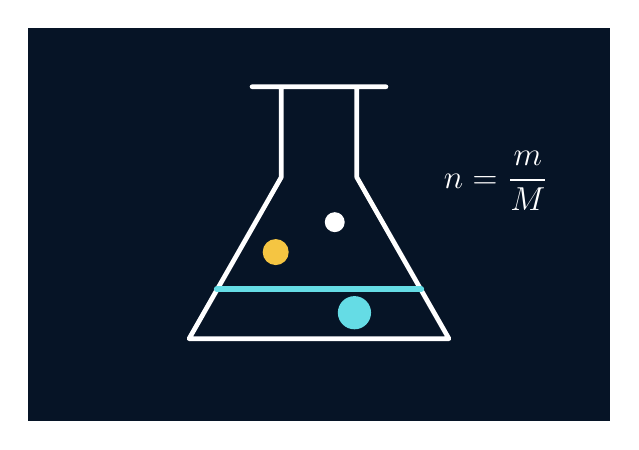
\begin{tikzpicture}[line cap=round,line join=round]
\fill[nostranavy] (-3.7,-2.5) rectangle (3.7,2.5);
\draw[white,line width=1.7pt] (-.85,1.75)--(.85,1.75) (-.48,1.75)--(-.48,.60)--(-1.65,-1.45)--(1.65,-1.45)--(.48,.60)--(.48,1.75);
\draw[nostracyan,line width=2pt] (-1.30,-.82)--(1.30,-.82);
\fill[nostragold] (-.55,-.35) circle (4.7pt); \fill[nostracyan] (.45,-1.12) circle (6pt); \fill[white] (.20,.03) circle (3.6pt);
\node[white,font=\bfseries\large] at (2.25,.55) {$n=\dfrac{m}{M}$};
\end{tikzpicture}
\end{document}
